\section{Experimental Results and Empirical Analysis}
\label{sec:results}

We evaluate the empirical performance of sub-2B open-weight safety judges on the reconciled $N=50$ conversation benchmark from Google DICES-350. Following the experimental formulation established in Section~\ref{sec:methodology_experimental_setup}, our evaluation addresses three central dimensions: (i) pointwise and ordinal approximation of continuous human consensus ($h_{\text{primary}}$), (ii) probability calibration under decile binning, and (iii) inter-judge disagreement ($\Delta$) as an empirical correlate of ensemble prediction error.

\subsection{Overall Judge Performance}
\label{subsec:overall_performance}

Table~\ref{tab:main_results} presents the consolidated performance matrix across all four evaluated systems: \texttt{Qwen2.5-0.5B-Instruct}, \texttt{SmolLM2-1.7B-Instruct}, the unweighted Two-Judge Ensemble ($P_{\text{ens}}$), and the held-out 5-fold out-of-fold (OOF) prevalence baseline.

\begin{table*}[t]
\centering
\caption{Consolidated Evaluation Performance Matrix on Google DICES-350 ($N=50$)}
\label{tab:main_results}
\renewcommand{\arraystretch}{1.2}
\setlength{\tabcolsep}{5pt}
\begin{tabular}{lccccccccc}
\toprule
\textbf{Evaluator System} & \textbf{Mean Pred.} ($\bar{P}\pm s$) & \textbf{MAE} $\downarrow$ & \textbf{RMSE} $\downarrow$ & \textbf{Soft MSE} $\downarrow$ & \textbf{ECE}$_{10}$ $\downarrow$ & \textbf{Pop. Bins} & \textbf{Pearson} $r$ & \textbf{Spearman} $\rho$ & \textbf{AUROC} $\uparrow$ \\
\midrule
Qwen2.5-0.5B-Instruct & $0.7509 \pm 0.1884$ & $0.4152$ & $0.4693$ & $0.2202$ & $0.4128$ & $8/10$ & $0.4812$ ($p=4.0\times 10^{-4}$) & $0.5680$ ($p=1.7\times 10^{-5}$) & $\mathbf{0.7529}$ \\
SmolLM2-1.7B-Instruct & $0.2531 \pm 0.0279$ & $\mathbf{0.1734}$ & $0.2505$ & $0.0628$ & $0.0850$ & $2/10$ & $0.2743$ ($p=0.0539$) & $0.3929$ ($p=0.0048$) & $0.6690$ \\
Two-Judge Ensemble (Equal-Weight) & $0.5020 \pm 0.0984$ & $0.2464$ & $0.2669$ & $0.0713$ & $0.1639$ & $6/10$ & $\mathbf{0.4992}$ ($p=2.2\times 10^{-4}$) & $\mathbf{0.5903}$ ($p=6.4\times 10^{-6}$) & $0.7517$ \\
\midrule
Prevalence Baseline (5-Fold OOF) & $0.3398 \pm 0.0144$ & $0.1983$ & $\mathbf{0.2454}$ & $\mathbf{0.0602}$ & $0.0017^*$ & $1/10$ & $-0.2353$ ($p=0.1001$) & $-0.1941$ ($p=0.1769$) & N/A$^\dagger$ \\
\bottomrule
\end{tabular}
\begin{flushleft}
\footnotesize
$^*$The 5-fold OOF prevalence baseline yields $\text{ECE}=0.0017$ across its single populated bin $[0.3, 0.4)$ ($(\bar{p}, \bar{h})=(0.3398, 0.3381)$); the degenerate in-sample constant reference yields $\text{ECE}=0.0000$ and is omitted. Both reflect single-bin aggregation artifacts rather than calibrated safety discrimination.\\
$^\dagger$As a constant-style reference within folds, the prevalence baseline cannot perform threshold-based ranking; AUROC is mathematically uninformative. Reported prediction standard deviations ($s$) denote sample standard deviations ($\text{ddof}=1$; corresponding population values $\sigma$ are $0.1865$, $0.0276$, $0.0975$, and $0.0142$).
\end{flushleft}
\end{table*}

The empirical data reveal a pronounced structural divergence between the two constituent architectures, highlighting distinct inductive biases in sub-2B language models:
\begin{enumerate}
    \item \textbf{Polarization of Single Judges:} \texttt{Qwen2.5-0.5B-Instruct} operates as an aggressive, risk-averse detector, yielding a high mean predicted unsafe probability ($\bar{P}=0.7509$, $s=0.1884$). This pronounced positive bias produces severe pointwise approximation penalties ($\text{MAE}=0.4152$, $\text{Soft MSE}=0.2202$). Conversely, \texttt{SmolLM2-1.7B-Instruct} exhibits severe low-score probability compression ($\bar{P}=0.2531$, $s=0.0279$), clustering tightly below the empirical human benchmark mean ($\bar{h}=0.3381$).
    \item \textbf{Ensemble Error Moderation:} The unweighted Two-Judge Ensemble achieves substantial pointwise error reductions relative to Qwen, reducing MAE by $40.6\%$ ($0.4152 \to 0.2464$) and Soft MSE by $67.6\%$ ($0.2202 \to 0.0713$).
    \item \textbf{Absence of Universal Dominance:} Crucially, the ensemble does not dominate across all metrics. SmolLM2 achieves the lowest MAE among the three judges ($0.1734$), and the 5-fold OOF prevalence baseline achieves lower RMSE ($0.2454$) and lower Soft MSE ($0.0602$) than the ensemble ($0.2669$ and $0.0713$, respectively).
\end{enumerate}

\subsection{Error and Soft-Target Agreement}
\label{subsec:error_agreement}

A central empirical insight of this investigation is the fundamental tension between pointwise prediction accuracy and ordinal ranking alignment when evaluating small models against continuous human distributions.

While SmolLM2 attains the lowest sample MAE ($0.1734$), its linear association with human consensus is weak and marginally non-significant ($r=0.2743$, $p=0.0539$). Its Spearman rank correlation ($\rho=0.3929$, $p=0.0048$) is notably degraded compared to Qwen. SmolLM2's low pointwise error is primarily a consequence of variance collapse: by concentrating $96\%$ of its predictions within the single decile $[0.2, 0.3)$, it anchors adjacent to the bulk of the human target distribution, effectively minimizing absolute residuals without executing granular safety distinctions.

Conversely, Qwen exhibits substantial ordinal acuity, capturing a Spearman rank correlation of $\rho=0.5680$ ($p=1.69\times 10^{-5}$) and Pearson $r=0.4812$ ($p=4.04\times 10^{-4}$), despite its severe pointwise error. Qwen successfully preserves relative safety orderings across diverse adversarial prompts, even though its raw softmax probabilities suffer from extreme upward scaling.

By combining these polarized predictors, the Two-Judge Ensemble captures the strongest monotonic and linear alignment with human consensus across all evaluated models, achieving Pearson $r=\mathbf{0.4992}$ ($p=2.24\times 10^{-4}$) and Spearman $\rho=\mathbf{0.5903}$ ($p=6.43\times 10^{-6}$). The ensemble effectively leverages Qwen's rank discriminability while exploiting SmolLM2's low baseline anchoring to temper runaway probability magnitude.

Nevertheless, the performance of the held-out prevalence baseline provides a vital methodological check: by outputting the out-of-fold training mean ($\bar{P}=0.3398$), this trivial non-learning heuristic achieves $\text{Soft MSE}=0.0602$, outperforming both the ensemble and SmolLM2 on squared error. This confirms that quadratic loss functions (such as Brier score~\cite{brier1950verification} and MSE) strongly reward prevalence-proximal conservatism, demonstrating that low MSE in isolation cannot be taken as evidence of learned conversational safety judgment.

\begin{figure}[t]
    \centering
    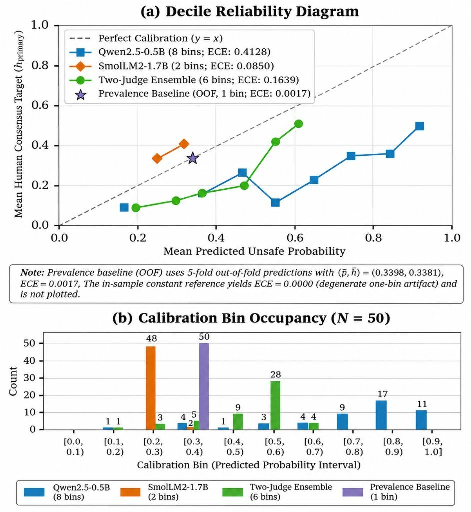
\includegraphics[width=\columnwidth]{figures/fig3_reliability.pdf}
    \caption{Empirical calibration analysis on $N=50$ conversations from Google DICES-350. (a) Decile reliability diagram plotting mean human target ($h_{\text{primary}}$) against mean predicted unsafe probability across 10 uniform bins. Markers are plotted only for populated bins; solid lines connect adjacent populated bins. The diagonal dashed line denotes perfect calibration ($y=x$). Qwen (blue squares, 8 bins) and the Ensemble (green circles, 6 bins) consistently overpredict across all populated bins. SmolLM2 (orange diamonds, 2 bins) underpredicts across both populated bins. The 5-fold OOF prevalence baseline (purple star, 1 bin) falls near the diagonal at $(0.3398, 0.3381)$ with $\text{ECE}=0.0017$. (b) Decile bin occupancy histogram showing extreme sample sparsity: Qwen spans 8 bins (peaking at $[0.8, 0.9)$ with 17 items); SmolLM2 is compressed into 2 bins (48 items in $[0.2, 0.3)$); the Ensemble spans 6 bins (peaking at $[0.5, 0.6)$ with 28 items); and the prevalence baseline collapses into a single bin ($[0.3, 0.4)$, 50 items).}
    \label{fig:reliability}
\end{figure}

\subsection{Calibration and Prediction Distribution}
\label{subsec:calibration}

Fig.~\ref{fig:reliability} illustrates the decile reliability diagram and corresponding sample occupancy distributions across all evaluators. Decile bins are defined uniformly over $[0, 1]$ with width $0.1$. 

The calibration analysis exposes marked differences in directional miscalibration and occupancy density:
\begin{itemize}
    \item \textbf{Directional Miscalibration:} In Panel~(a), all 8 populated bins for Qwen lie strictly below the diagonal identity line ($y=x$), demonstrating systematic, uniform overprediction of conversational hazard. Similarly, all 6 populated bins for the Two-Judge Ensemble lie below the identity line, confirming that while ensembling moderates probability magnitude, it remains an overpredicting evaluator. In sharp contrast, SmolLM2 underpredicts in both of its populated bins: in bin $[0.2, 0.3)$ ($48$ items), its mean prediction is $0.2519$ against a mean human target of $0.3355$; in bin $[0.3, 0.4)$ ($2$ items), its mean prediction is $0.3160$ against a mean target of $0.4077$.
    \item \textbf{Occupancy Sparsity and ECE Distortion:} Panel~(b) demonstrates that reported ECE values must not be interpreted as interchangeable scalar indicators of calibration quality. Qwen populates 8 separate bins spanning $[0.1, 1.0]$, exhibiting genuine dispersion with high calibration error ($\text{ECE}_{10}=0.4128$). The Two-Judge Ensemble occupies 6 bins spanning $[0.1, 0.7]$, achieving an intermediate Expected Calibration Error~\cite{guo2017calibration} ($\text{ECE}_{10}=0.1639$). In contrast, SmolLM2's low $\text{ECE}_{10}$ ($0.0850$) is an artifact of extreme bin compression, with 48 of 50 conversations clustered into a single interval.
    \item \textbf{Prevalence Baseline Single-Bin Artifact:} The 5-fold OOF prevalence baseline achieves an apparent $\text{ECE}_{10}$ of $0.0017$. Because its predictions vary only marginally across cross-validation folds ($s=0.0142$), all 50 items fall into the single decile $[0.3, 0.4)$, where the fold-average prediction ($0.3398$) aligns closely with the sample mean ($0.3381$). An in-sample constant reference achieves an ECE of identically $0.0000$. Interpreting this near-zero ECE as superior calibration would be entirely erroneous; it is a degenerate artifact of zero prediction variance.
\end{itemize}

\subsection{Majority-Label Discrimination}
\label{subsec:discrimination}

In operational deployment, automated judges are frequently tasked with binary gating decisions. To evaluate discriminative acuity independently of raw probability calibration, we map human soft consensus to the majority classification target:
\begin{equation}
    y_{\text{majority}, i} = \mathbf{1}(h_{\text{primary}, i} \ge 0.5)
\end{equation}
Within our reconciled $N=50$ sample, this partition yields $N_{\text{pos}}=11$ majority-unsafe conversations ($22\%$) and $N_{\text{neg}}=39$ majority-safe conversations ($78\%$), defining exactly $N_{\text{pos}} \times N_{\text{neg}} = 429$ positive-negative comparison pairs.

As detailed in Table~\ref{tab:main_results}, \texttt{Qwen2.5-0.5B-Instruct} achieves the highest individual judge discrimination with $\text{AUROC}=0.7529$ ($95\%$ stratified bootstrap CI: $[0.5944, 0.8881]$, $B=2,000$). \texttt{SmolLM2-1.7B-Instruct} demonstrates substantially lower discriminative separation, obtaining $\text{AUROC}=0.6690$ ($95\%$ CI: $[0.5116, 0.8159]$).

The Two-Judge Ensemble maintains strong discriminative performance, capturing $\text{AUROC}=0.7517$ ($95\%$ CI: $[0.6049, 0.8765]$). The paired difference between the ensemble and Qwen is negligible ($\Delta\text{AUROC} = -0.0012$, $95\%$ bootstrap CI: $[-0.0524, +0.0443]$). Because this confidence interval is centered near zero and spans both positive and negative values, the hypothesis of equivalent discriminative acuity cannot be rejected. Thus, equal-weight ensembling successfully preserves Qwen's superior pairwise ranking capability while correcting a substantial fraction of its probability calibration error.

\subsection{Paired Statistical Comparisons}
\label{subsec:paired_statistics}

To rigorously assess whether observed error differences between evaluators are statistically significant, we conduct formal paired hypothesis tests. Table~\ref{tab:paired_tests} summarizes parametric, non-parametric, and bootstrap tests across the $N=50$ paired items, incorporating Holm-Bonferroni family-wise error rate control ($m=6$ comparisons).

\begin{table*}[t]
\centering
\caption{Paired Statistical Comparisons and Hypothesis Tests on Evaluator Errors ($N=50$)}
\label{tab:paired_tests}
\renewcommand{\arraystretch}{1.2}
\setlength{\tabcolsep}{4.5pt}
\begin{tabular}{lcccccccc}
\toprule
\textbf{Paired Error Comparison} & \textbf{Mean Diff.} & \textbf{Paired} $t$ ($p_{\text{unadj}}$) & $p_{\text{Holm}}$ & \textbf{Wilcoxon} $W$ ($p_{\text{unadj}}$) & $W$ $p_{\text{Holm}}$ & \textbf{Sign Test} & \textbf{Item Boot 95\% CI} & \textbf{Rater Boot 95\% CI} \\
\midrule
Qwen vs Ensemble MAE & $+0.1688$ & $t=6.73$ ($1.7\times 10^{-8}$) & $8.7\times 10^{-8}$ & $146.5$ ($2.1\times 10^{-6}$) & $1.1\times 10^{-5}$ & $44\text{ wins } / 6\text{ losses}$ & $[+0.1181, +0.2153]$ & $[+0.1535, +0.1853]$ \\
Qwen vs Ensemble Soft MSE & $+0.1489$ & $t=7.74$ ($4.7\times 10^{-10}$) & $2.8\times 10^{-9}$ & $88.0$ ($3.1\times 10^{-9}$) & $1.9\times 10^{-8}$ & $44\text{ wins } / 6\text{ losses}$ & $[+0.1105, +0.1846]$ & $[+0.1314, +0.1660]$ \\
\midrule
SmolLM2 vs Ensemble MAE & $-0.0730$ & $t=-2.38$ ($0.0213$) & $0.0425^*$ & $427.0$ ($0.0421$) & $0.0843^\dagger$ & $36\text{ wins } / 14\text{ losses}$ & $[-0.1298, -0.0101]$ & $[-0.0935, -0.0355]$ \\
SmolLM2 vs Ensemble Soft MSE & $-0.0085$ & $t=-0.47$ ($0.6425$) & $0.6425^\dagger$ & $473.0$ ($0.1139$) & $0.1139^\dagger$ & $29\text{ wins } / 21\text{ losses}$ & $[-0.0414, +0.0290]$ & $[-0.0256, +0.0091]$ \\
\midrule
Qwen vs SmolLM2 MAE & $+0.2418$ & $t=4.61$ ($2.9\times 10^{-5}$) & $1.1\times 10^{-4}$ & $250.0$ ($1.8\times 10^{-4}$) & $5.5\times 10^{-4}$ & $40\text{ wins } / 10\text{ losses}$ & $[+0.1390, +0.3445]$ & $[+0.2198, +0.2529]$ \\
Qwen vs SmolLM2 Soft MSE & $+0.1575$ & $t=4.36$ ($6.6\times 10^{-5}$) & $2.0\times 10^{-4}$ & $253.0$ ($1.2\times 10^{-4}$) & $4.8\times 10^{-4}$ & $38\text{ wins } / 12\text{ losses}$ & $[+0.0867, +0.2282]$ & $[+0.1458, +0.1706]$ \\
\bottomrule
\end{tabular}
\begin{flushleft}
\footnotesize
$^*$Significant at family-wise $\alpha=0.05$. $^\dagger$Fails to achieve statistical significance after Holm-Bonferroni adjustment. Wins/losses denote item-level error comparisons. Item bootstrap employs $B=2,000$ resamples of conversations; Rater cluster bootstrap employs $B=1,000$ resamples over the 104 unique annotator clusters.
\end{flushleft}
\end{table*}

The hypothesis test results yield three critical methodological findings:
\begin{enumerate}
    \item \textbf{Ensemble Superiority over Qwen:} The error reduction achieved by the ensemble over Qwen is unambiguous and highly significant across all specifications. Both the parametric paired $t$-test ($t(49)=6.73$, $p_{\text{Holm}}=8.69\times 10^{-8}$, Cohen's $d_z=0.952$) and non-parametric Wilcoxon signed-rank test ($W=146.5$, $Z=-4.74$, $p_{\text{Holm}}=1.07\times 10^{-5}$, effect size $r=-0.670$) confirm large, robust gains. Item and rater cluster bootstraps both exclude zero by a wide margin.
    \item \textbf{Test-Sensitivity of SmolLM2 vs. Ensemble MAE:} SmolLM2's sample MAE advantage over the ensemble ($-0.0730$) is sensitive to the statistical test employed. A Shapiro-Wilk test on the paired MAE differences provides strong empirical evidence of departure from normality ($W=0.8776$, $p=9.47\times 10^{-5}$), which urges caution when interpreting parametric $t$-test inferences and motivates non-parametric validation. While the parametric $t$-test indicates significance after Holm adjustment ($p_{\text{unadj}}=0.0213$, $p_{\text{Holm}}=0.0425$) and the two-sided sign test indicates $36$ items favored SmolLM2 versus $14$ for the ensemble ($p=0.0026$), the non-parametric Wilcoxon test ($W=427.0$, $Z=-2.032$, unadjusted $p=0.0421$) yields an adjusted $p_{\text{Holm}}=\mathbf{0.0843}$. Thus, under conservative non-parametric family-wise error control, the MAE difference between SmolLM2 and the ensemble fails to achieve statistical significance at the standard $\alpha=0.05$ threshold.
    \item \textbf{Equivalence in Soft MSE:} In terms of quadratic soft error, SmolLM2 and the ensemble are statistically indistinguishable ($t(49)=-0.47$, $p_{\text{Holm}}=0.6425$; Wilcoxon $W=473.0$, unadjusted $p=0.1139$). Both the 2,000-replicate item bootstrap ($95\%$ CI: $[-0.0414, +0.0290]$) and 1,000-replicate rater cluster bootstrap ($95\%$ CI: $[-0.0256, +0.0091]$) span zero comfortably.
\end{enumerate}

\begin{figure}[t]
    \centering
    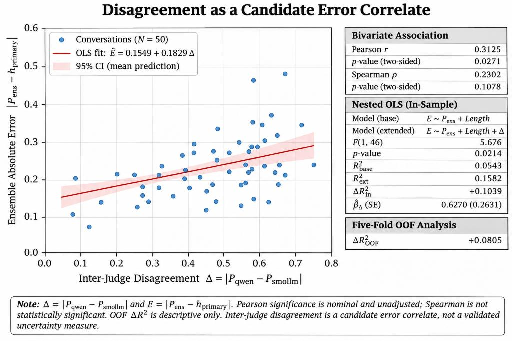
\includegraphics[width=\columnwidth]{figures/fig4_disagreement.pdf}
    \caption{Inter-judge disagreement ($\Delta$) as an empirical error correlate on $N=50$ conversations. Scatter plot displays item-level ensemble absolute error ($E_i = |P_{\text{ens}, i} - h_{\text{primary}, i}|$) versus inter-judge disagreement ($\Delta_i = |P_{\text{qwen}, i} - P_{\text{smollm}, i}|$). The solid red line denotes the bivariate OLS fit ($\hat{E} = 0.1549 + 0.1829\Delta$) with a $95\%$ mean-prediction confidence band (shaded pink). Right-hand panels summarize the statistical audit: bivariate linear association ($r=0.3125$, nominal $p=0.0271$; non-significant Spearman $\rho=0.2302$, $p=0.1078$), nested in-sample OLS diagnostics ($F(1, 46)=5.676$, $p=0.0214$, $\Delta R^2_{\text{in}}=+0.1039$, $\hat{\beta}_{\Delta}=0.6270$), and 5-fold cross-validation ($\Delta R^2_{\text{OOF}}=+0.0805$).}
    \label{fig:disagreement}
\end{figure}

\subsection{Disagreement and Error Association}
\label{subsec:disagreement_analysis}

A central hypothesis of TrustEval is that inter-judge disagreement ($\Delta_i = |P_{\text{qwen}, i} - P_{\text{smollm}, i}|$) between architecturally diverse small models carries informative signal regarding ensemble prediction error ($E_i = |P_{\text{ens}, i} - h_{\text{primary}, i}|$). Fig.~\ref{fig:disagreement} provides the empirical evaluation of this relationship.

\subsubsection{Bivariate Correlation Analysis}
Across the 50 evaluated conversations, inter-judge disagreement exhibits a positive linear correlation with ensemble absolute error: Pearson $r=0.3125$ ($p=0.0271$). However, this nominal significance does not hold under monotonic rank evaluation: the Spearman rank correlation is $\rho=0.2302$ ($p=0.1078$). The divergence between Pearson and Spearman coefficients demonstrates that while high-disagreement items tend to exhibit larger average absolute errors, the item-level mapping is not strictly monotonic; substantial error variance persists at intermediate and low disagreement levels.

\subsubsection{Nested OLS Regression}
To test whether $\Delta$ contributes unique predictive power beyond trivial conversation covariates, we estimate nested ordinary least squares (OLS) regression models. The baseline model controls for predicted ensemble probability magnitude and conversation text length:
\begin{equation}
    E_i = \beta_0 + \beta_1 P_{\text{ens}, i} + \beta_2 \text{Length}_i + \epsilon_i
\end{equation}
This baseline specification yields an in-sample coefficient of determination of $R^2_{\text{base}} = 0.0543$.

Extending the specification to include inter-judge disagreement:
\begin{equation}
    E_i = \beta_0 + \beta_1 P_{\text{ens}, i} + \beta_2 \text{Length}_i + \beta_3 \Delta_i + \epsilon_i
\end{equation}
increases the explained variance to $R^2_{\text{ext}} = 0.1582$, representing an incremental in-sample gain of $\Delta R^2_{\text{in}} = +0.1039$. In this extended specification, the estimated coefficient for disagreement is positive and statistically significant: $\hat{\beta}_{\Delta} = 0.6270$ ($\text{SE} = 0.2631$). A partial $F$-test confirms the significance of the incremental variance: $F(1, 46) = 5.676$ ($p = 0.0214$).

\subsubsection{Out-of-Fold Generalization}
To evaluate out-of-sample stability within the constraints of our 50-item sample, we conduct 5-fold cross-validation using folds stratified on $y_{\text{majority}}$. The baseline model achieves an out-of-fold generalization of $R^2_{\text{base, OOF}} = 0.0298$, whereas the extended model achieves $R^2_{\text{ext, OOF}} = 0.1103$, yielding a descriptive out-of-fold increment of $\Delta R^2_{\text{OOF}} = +0.0805$.

\subsubsection{Scientific Interpretation and Constraints}
We explicitly qualify the interpretation of these findings:
\begin{itemize}
    \item \textbf{Candidate Correlate, Not Calibrated Uncertainty:} Disagreement $\Delta$ is an empirical \textit{candidate correlate} of ensemble error; it is not a mathematically formal or calibrated epistemic uncertainty estimate.
    \item \textbf{Low Disagreement Does Not Guarantee Correctness:} Inspection of the lower-left quadrant of Fig.~\ref{fig:disagreement} demonstrates that several items with low inter-judge disagreement ($\Delta < 0.20$) nevertheless incur ensemble errors exceeding $0.20$. Low disagreement can occur when both sub-2B models share a common failure mode or identical systemic blind spot—a plausible explanation for these observed counterexamples. Consequently, low disagreement cannot be treated as a guarantee of correctness in safety-critical governance.
    \item \textbf{Exploratory Sample Scope:} While the nested partial $F$-test is statistically significant ($p=0.0214$), the total sample of $N=50$ conversations remains exploratory. Out-of-fold improvements must be interpreted as descriptive indicators rather than definitive proof of cross-domain generalization.
\end{itemize}
